\section{Results}

In this section we present the numerical results obtained for the Poisson problem model using both linear (CST) and quadratic (LST) triangular elements. We generate a sequence of uniform and geometrically graded meshes (controlled by the progression parameter $r$) and assemble the corresponding finite‐element systems by exact integration of the element stiffness matrices. After enforcing homogeneous Dirichlet conditions, we solve each sparse linear system to obtain the discrete solution \(u_h\). We then compute the energy‐norm error \(\|u - u_h\|_{H^1(\Omega)}\) against the known analytic solution and plot its decay versus the mesh size \(h\) on a log–log scale. By fitting a straight line to these data, we extract the observed convergence rates and compare them to the theoretical predictions of \(\mathcal{O}(h^1)\) for CST and \(\mathcal{O}(h^2)\) for LST. Tables and figures below summarize these findings for both uniform and graded discretizations.  

\subsection{CST annalysis}

\begin{figure}[H]
\centering
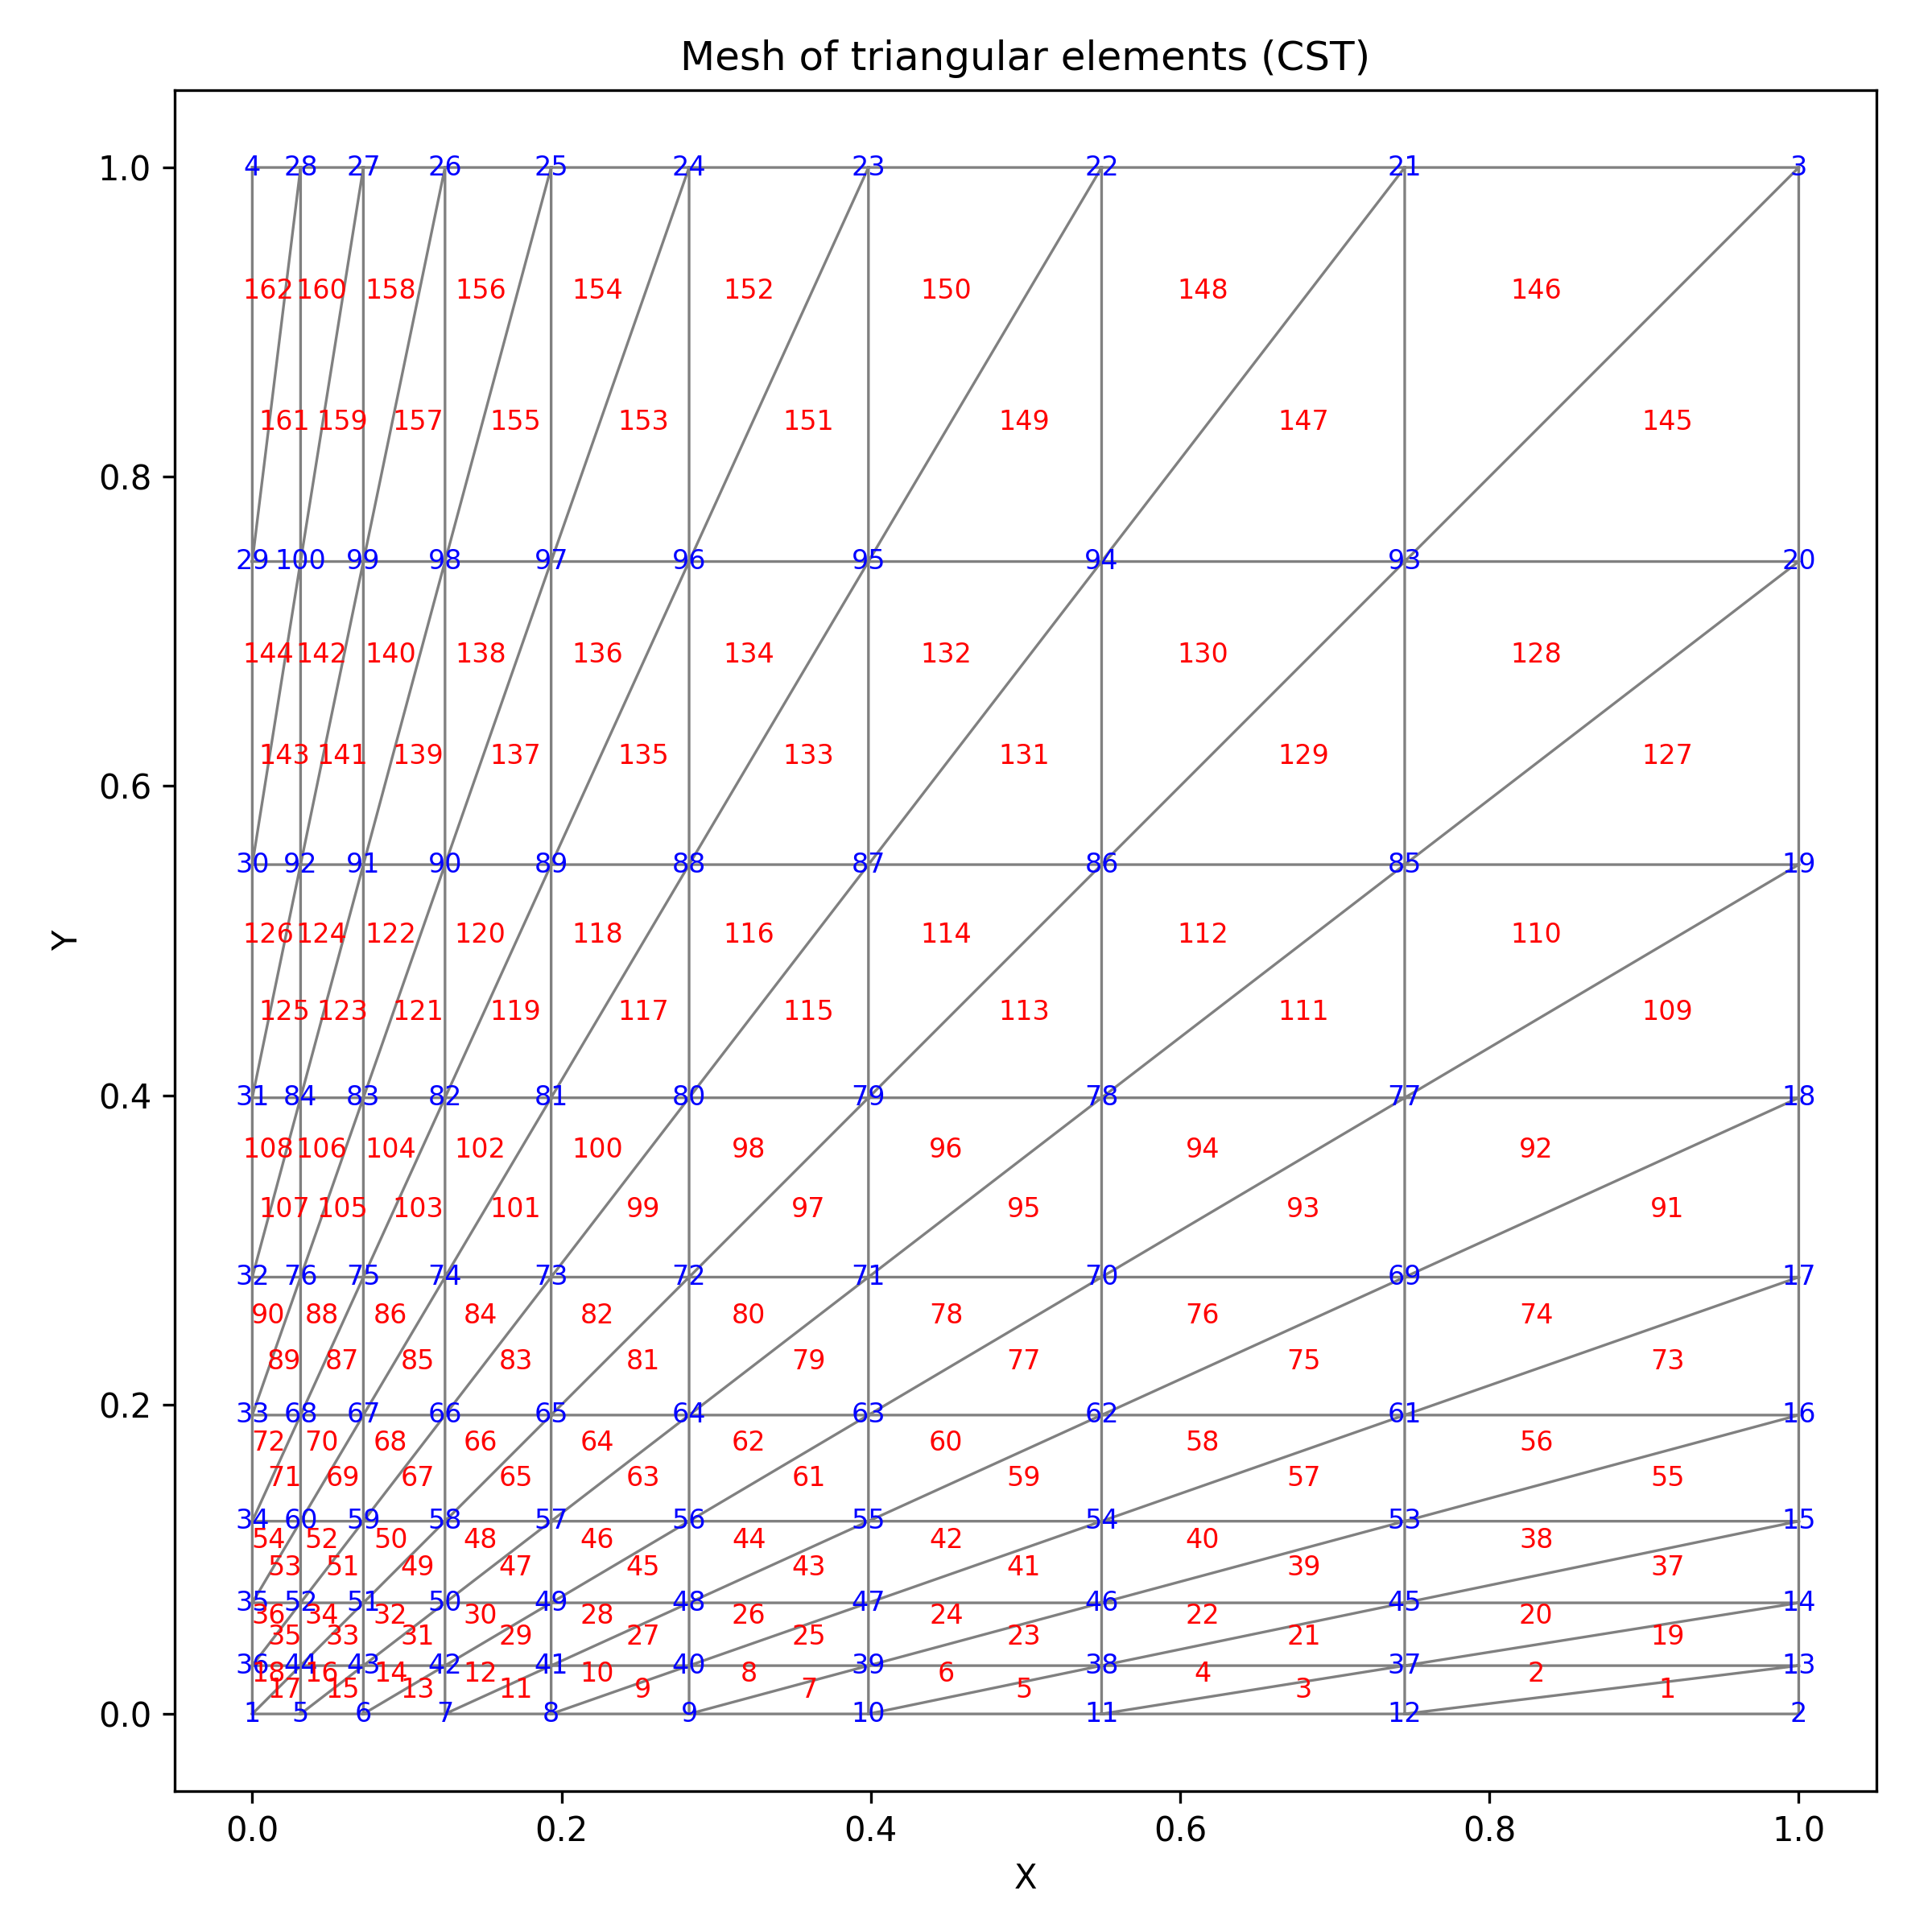
\includegraphics[width=0.4\textwidth]{GRAFICOS/CST/CST_mesh_plot.png}
\caption{CST Mesh}
\label{fig:cst_results}
\end{figure}

\begin{figure}[H]
  \centering
  \begin{subfigure}[b]{0.48\textwidth}
    \centering
    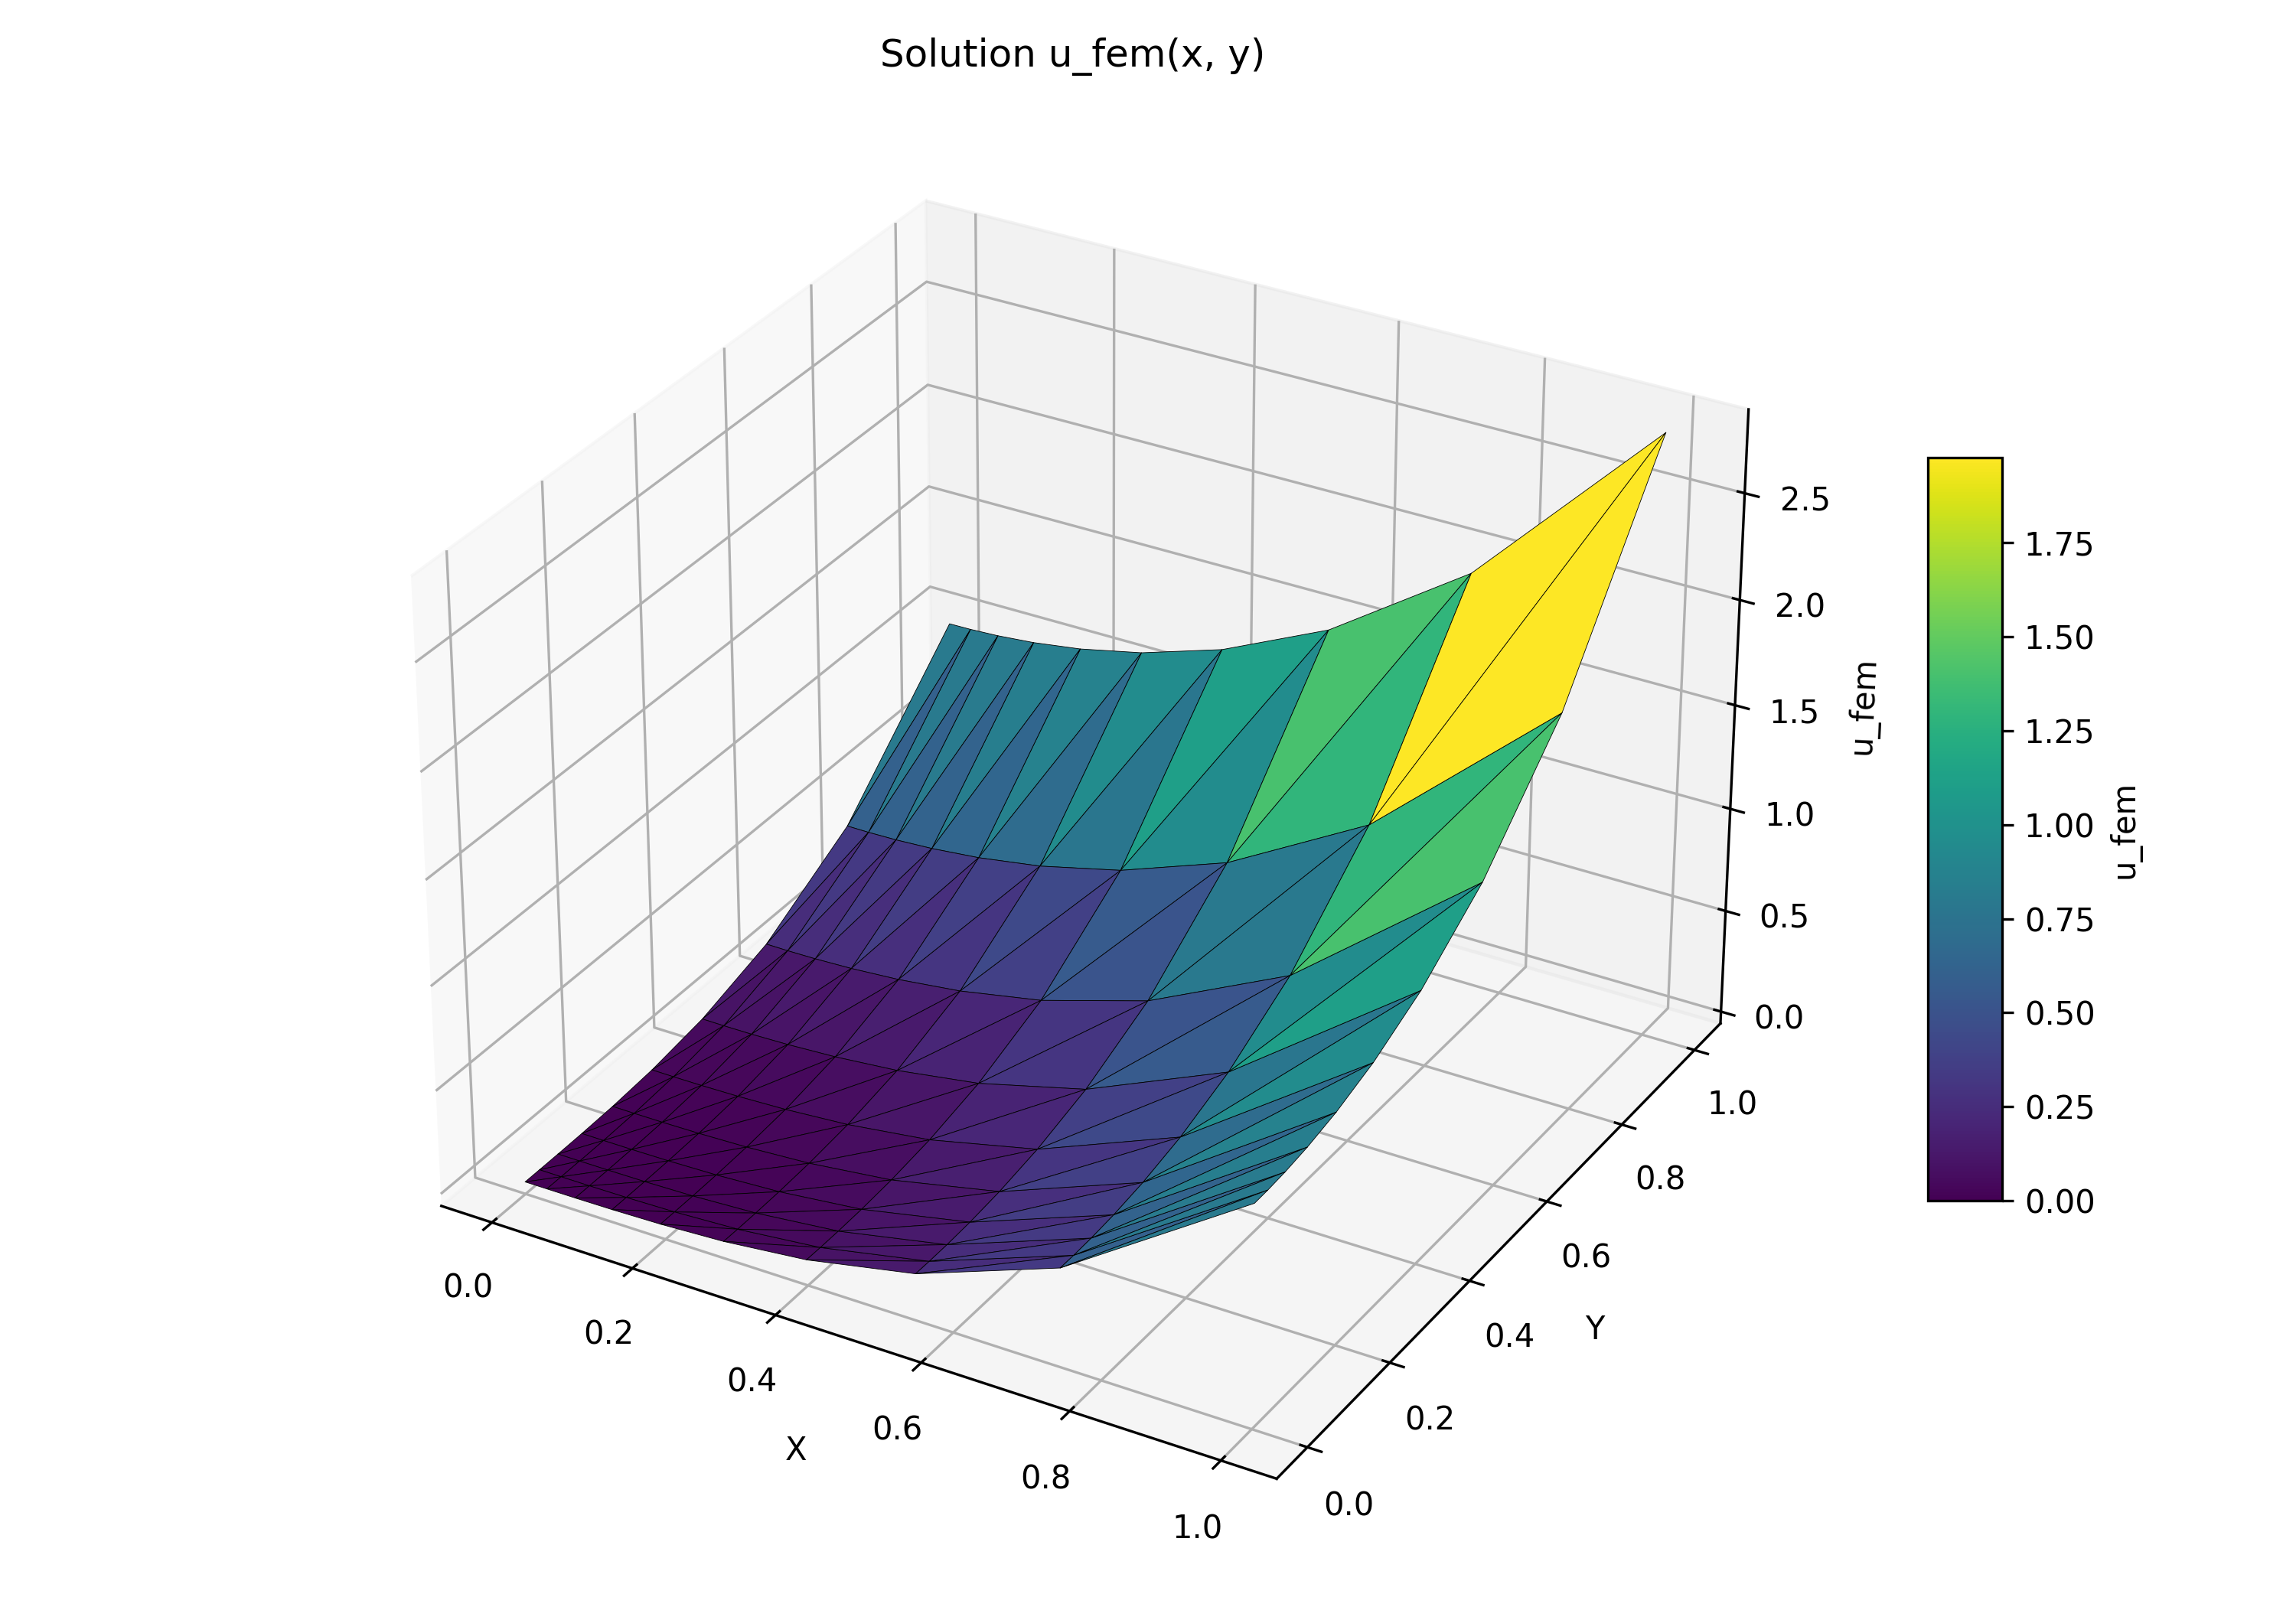
\includegraphics[width=\textwidth]{GRAFICOS/CST/CST_u_fem_sol_surface_plot.png}
    \caption{Discrete solution \(u_h\) for CST}
    \label{fig:cst_u_fem_sol}
  \end{subfigure}
  \hfill
  \begin{subfigure}[b]{0.48\textwidth}
    \centering
    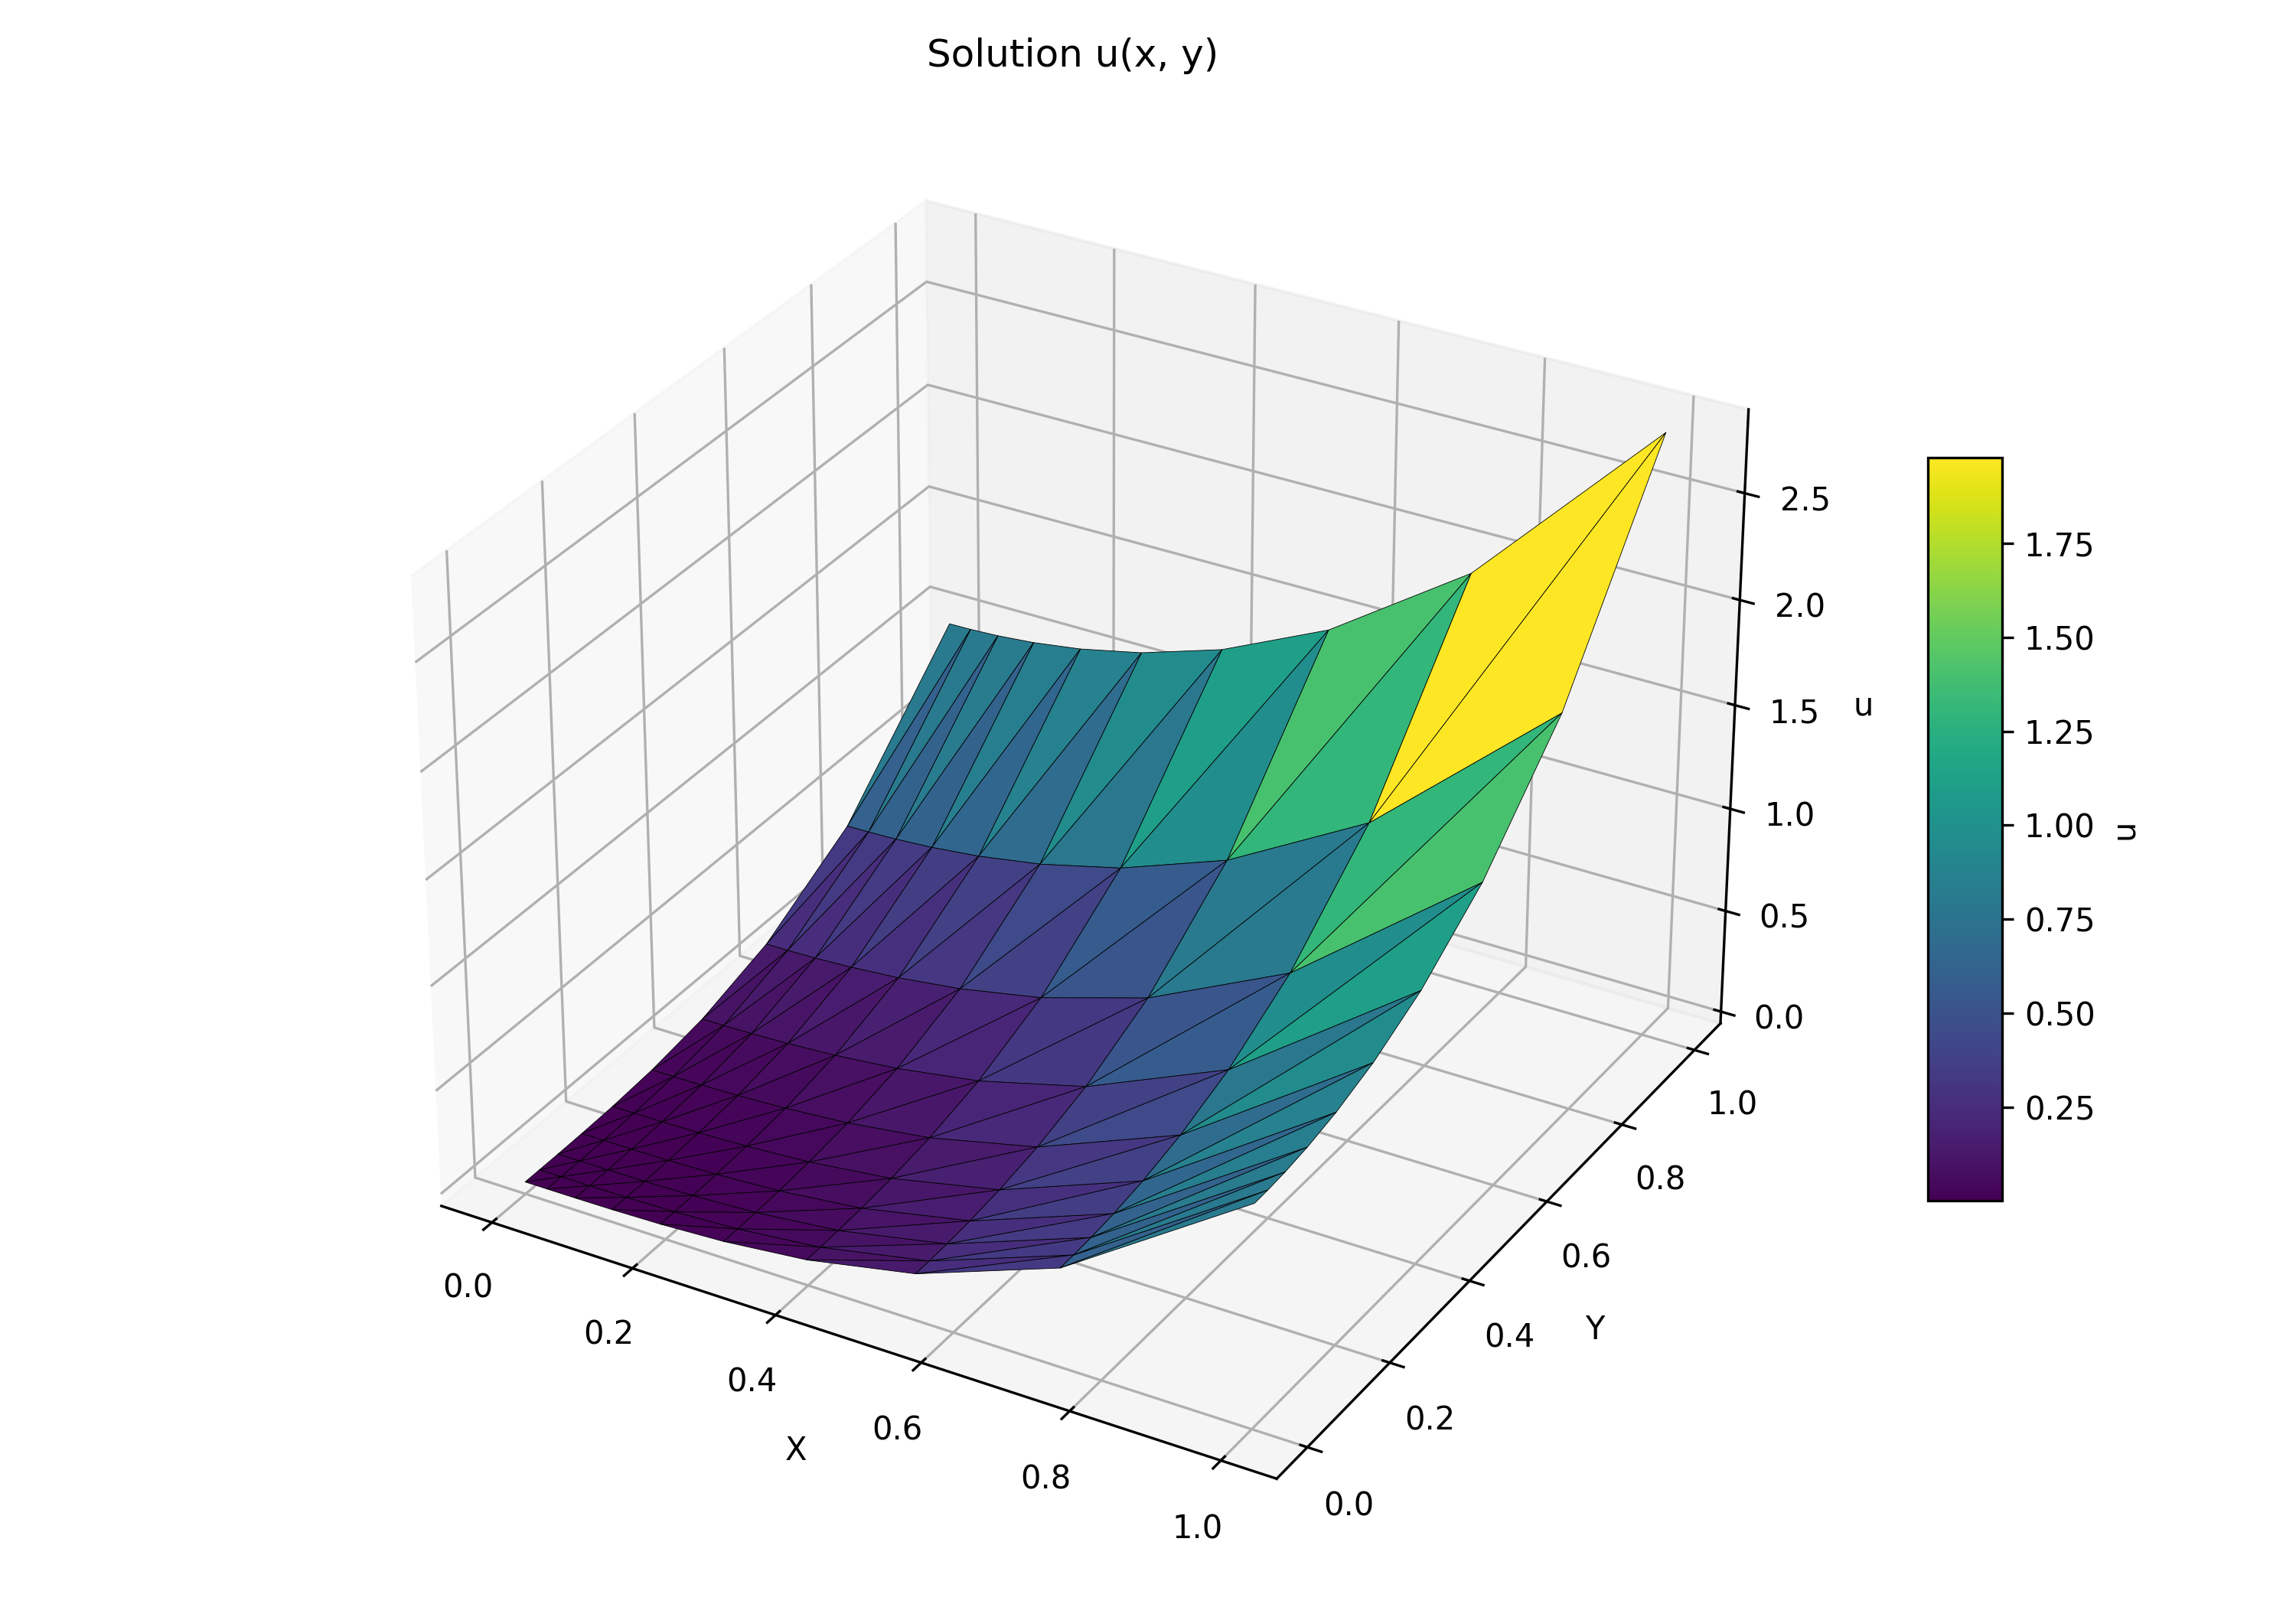
\includegraphics[width=\textwidth]{GRAFICOS/CST/CST_u_sol_surface_plot.png}
    \caption{Analytic solution \(u\) for CST}
    \label{fig:cst_error_plot}
  \end{subfigure}
  \caption{Comparison of the finite‐element discrete solution \(u_h\) and the analytic solution \(u\) for CST elements.}
  \label{fig:cst_comparison}
\end{figure}

\begin{figure}[H]
\centering
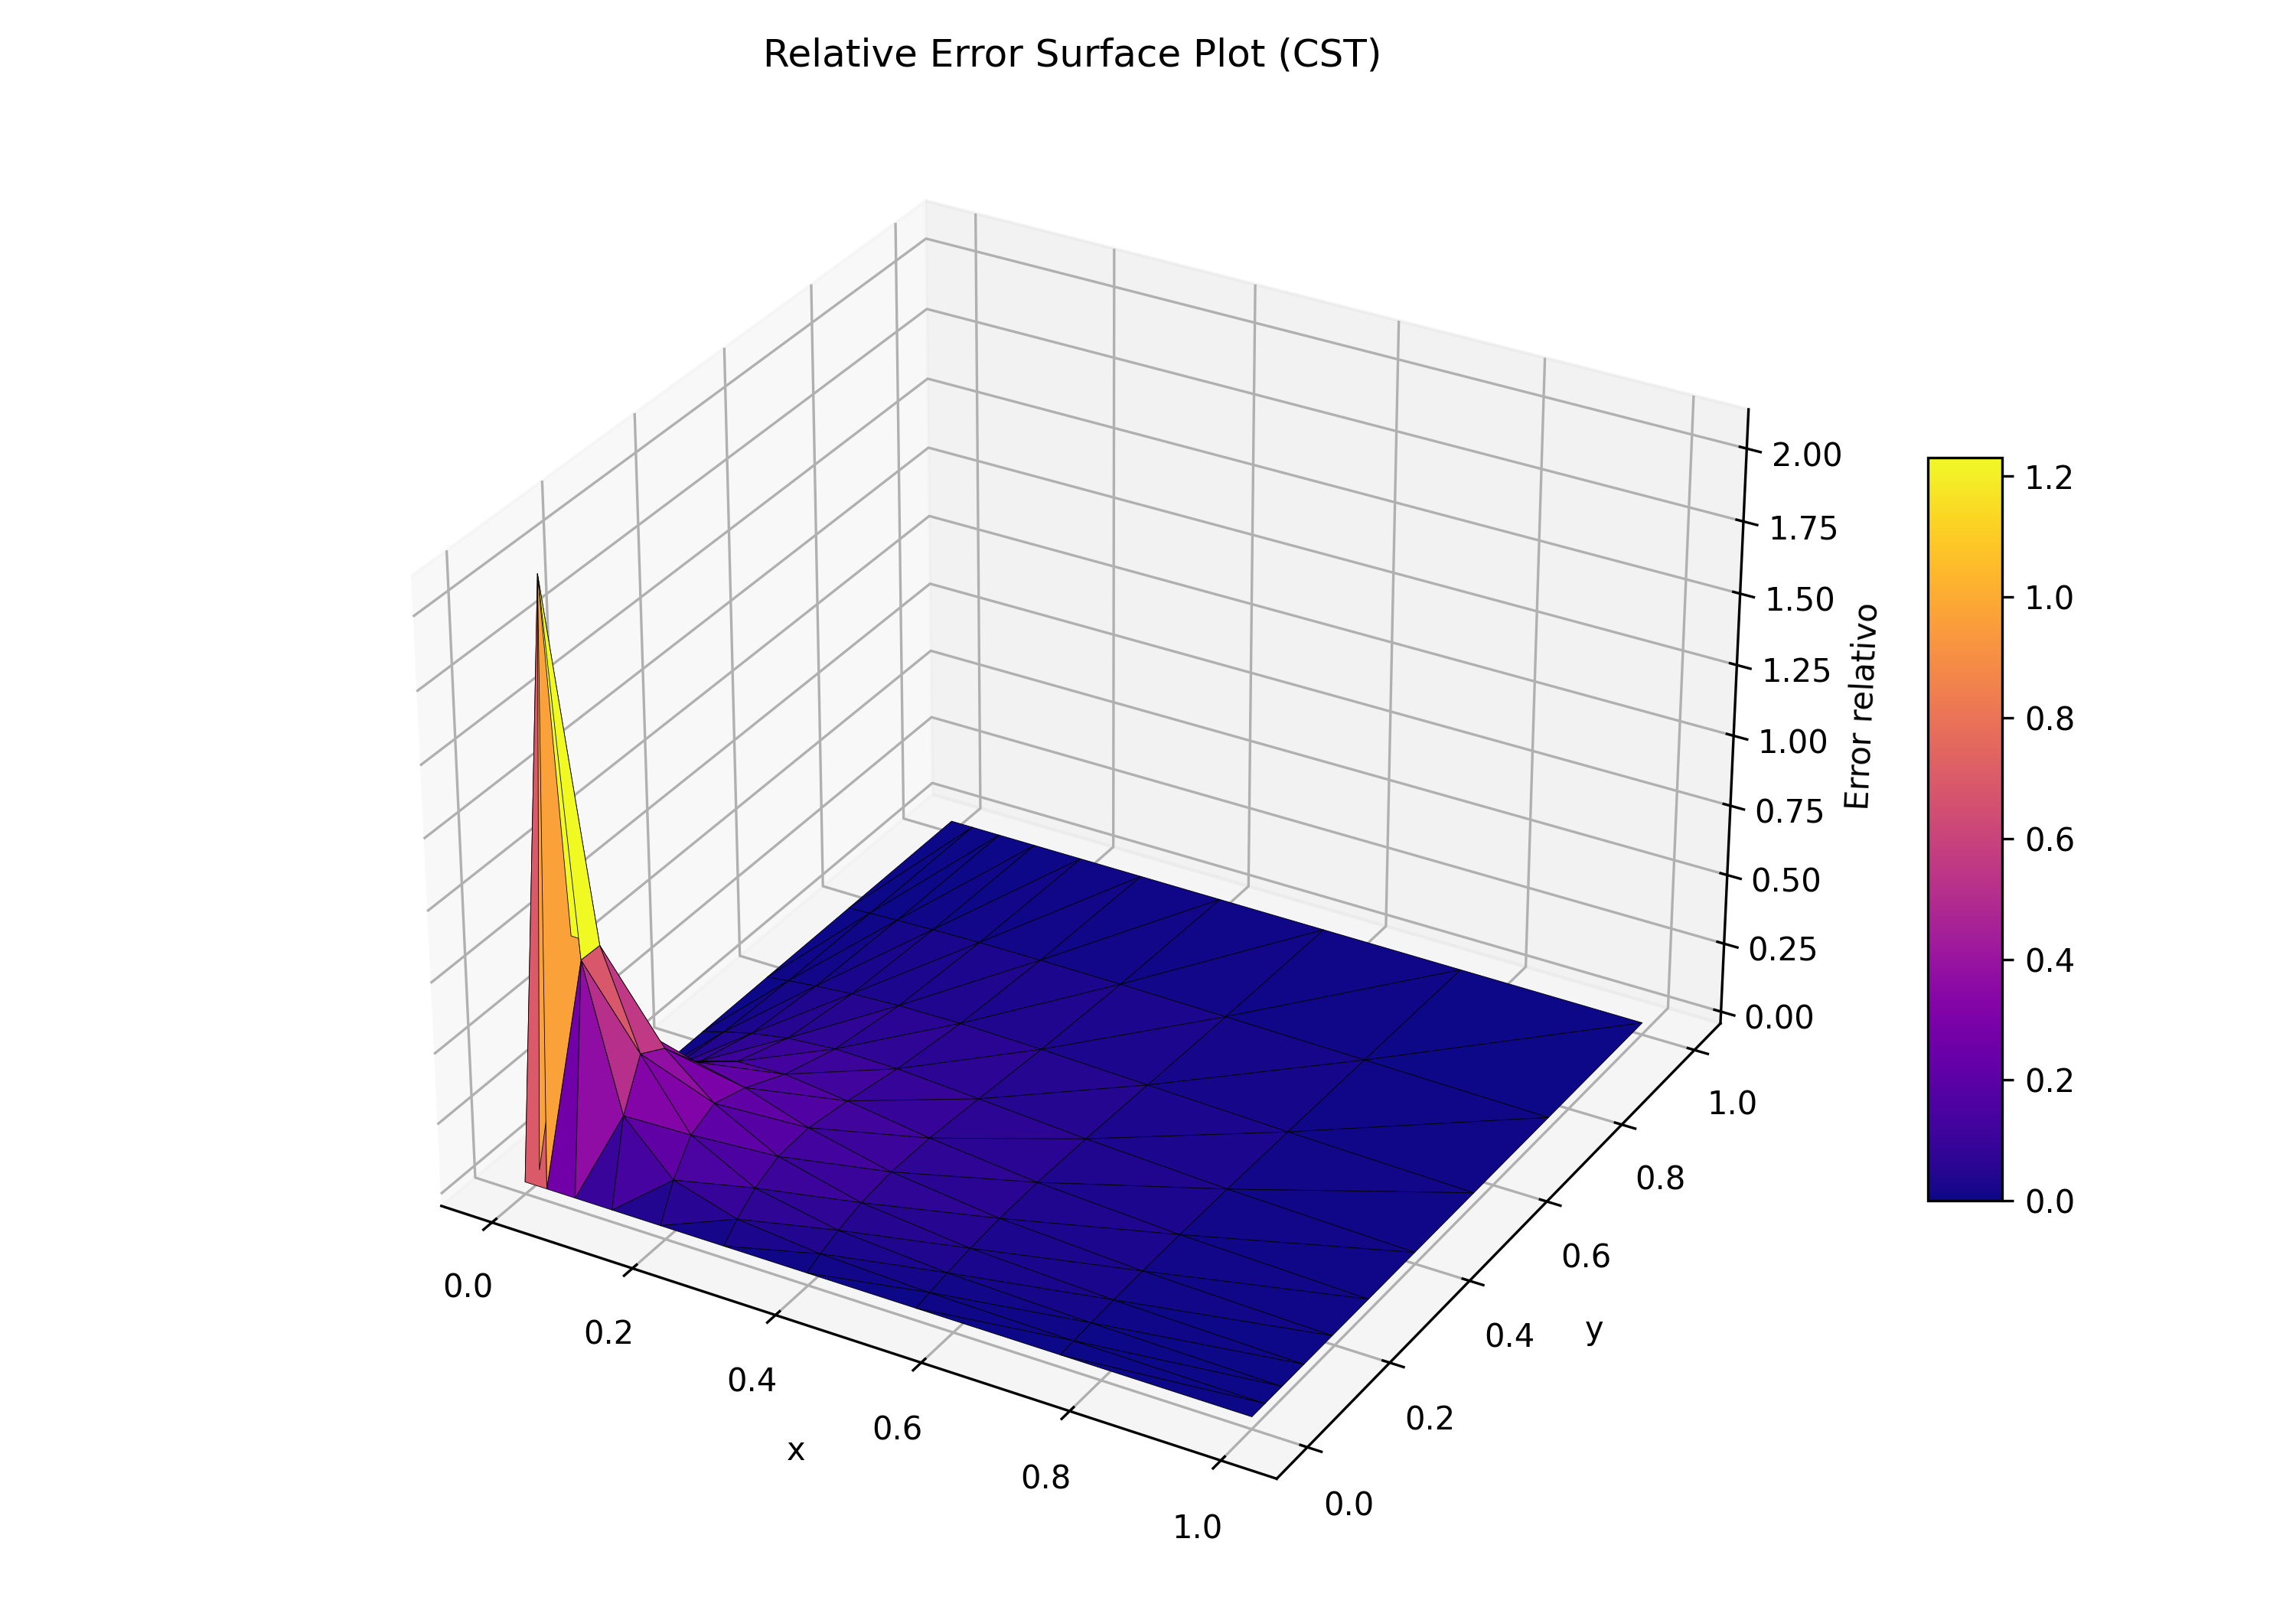
\includegraphics[width=0.6\textwidth]{GRAFICOS/CST/CST_relative_error_surface_plot.png}
\caption{Relative error \(\|u - u_h\|_{H^1(\Omega)}\) for CST elements}
\label{fig:cst_error_vs_h}
\end{figure}


\subsection{LST annalysis}

\begin{figure}[H]
\centering
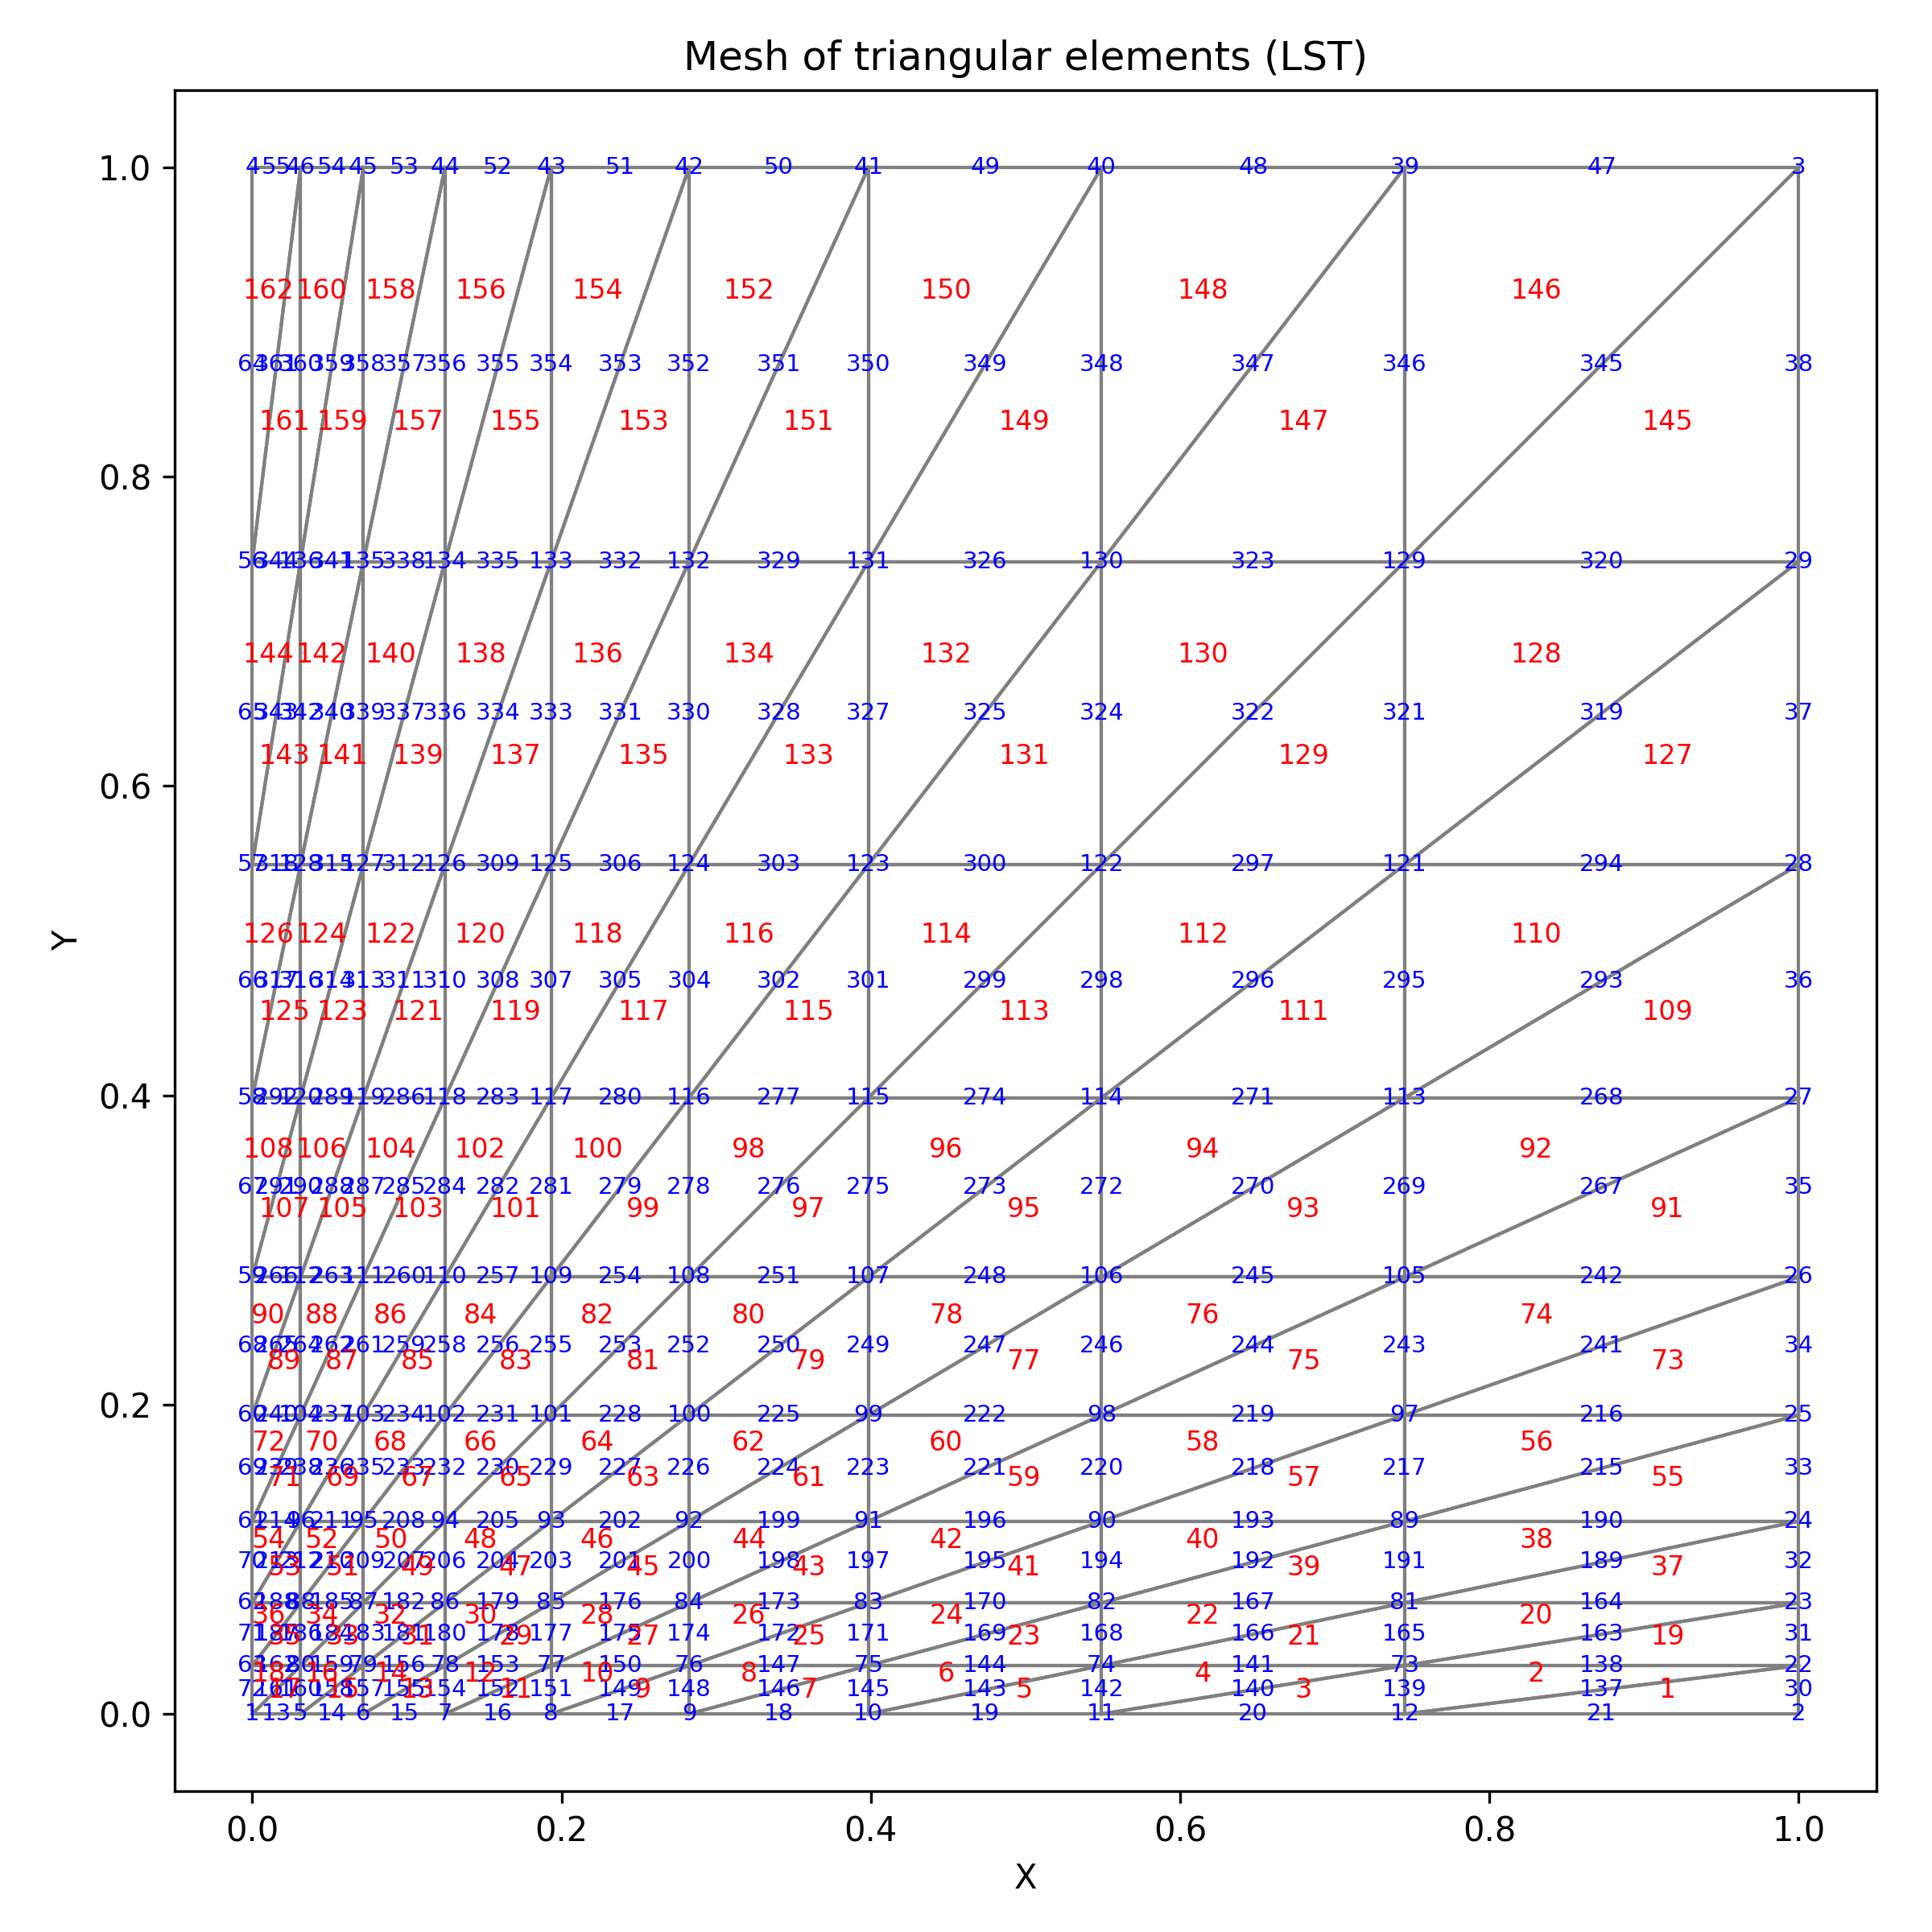
\includegraphics[width=0.4\textwidth]{GRAFICOS/LST/LST_mesh_plot.png}
\caption{LST Mesh}
\label{fig:lst_results}
\end{figure}

\begin{figure}[H]
\centering
\begin{subfigure}[b]{0.48\textwidth}
    \centering
    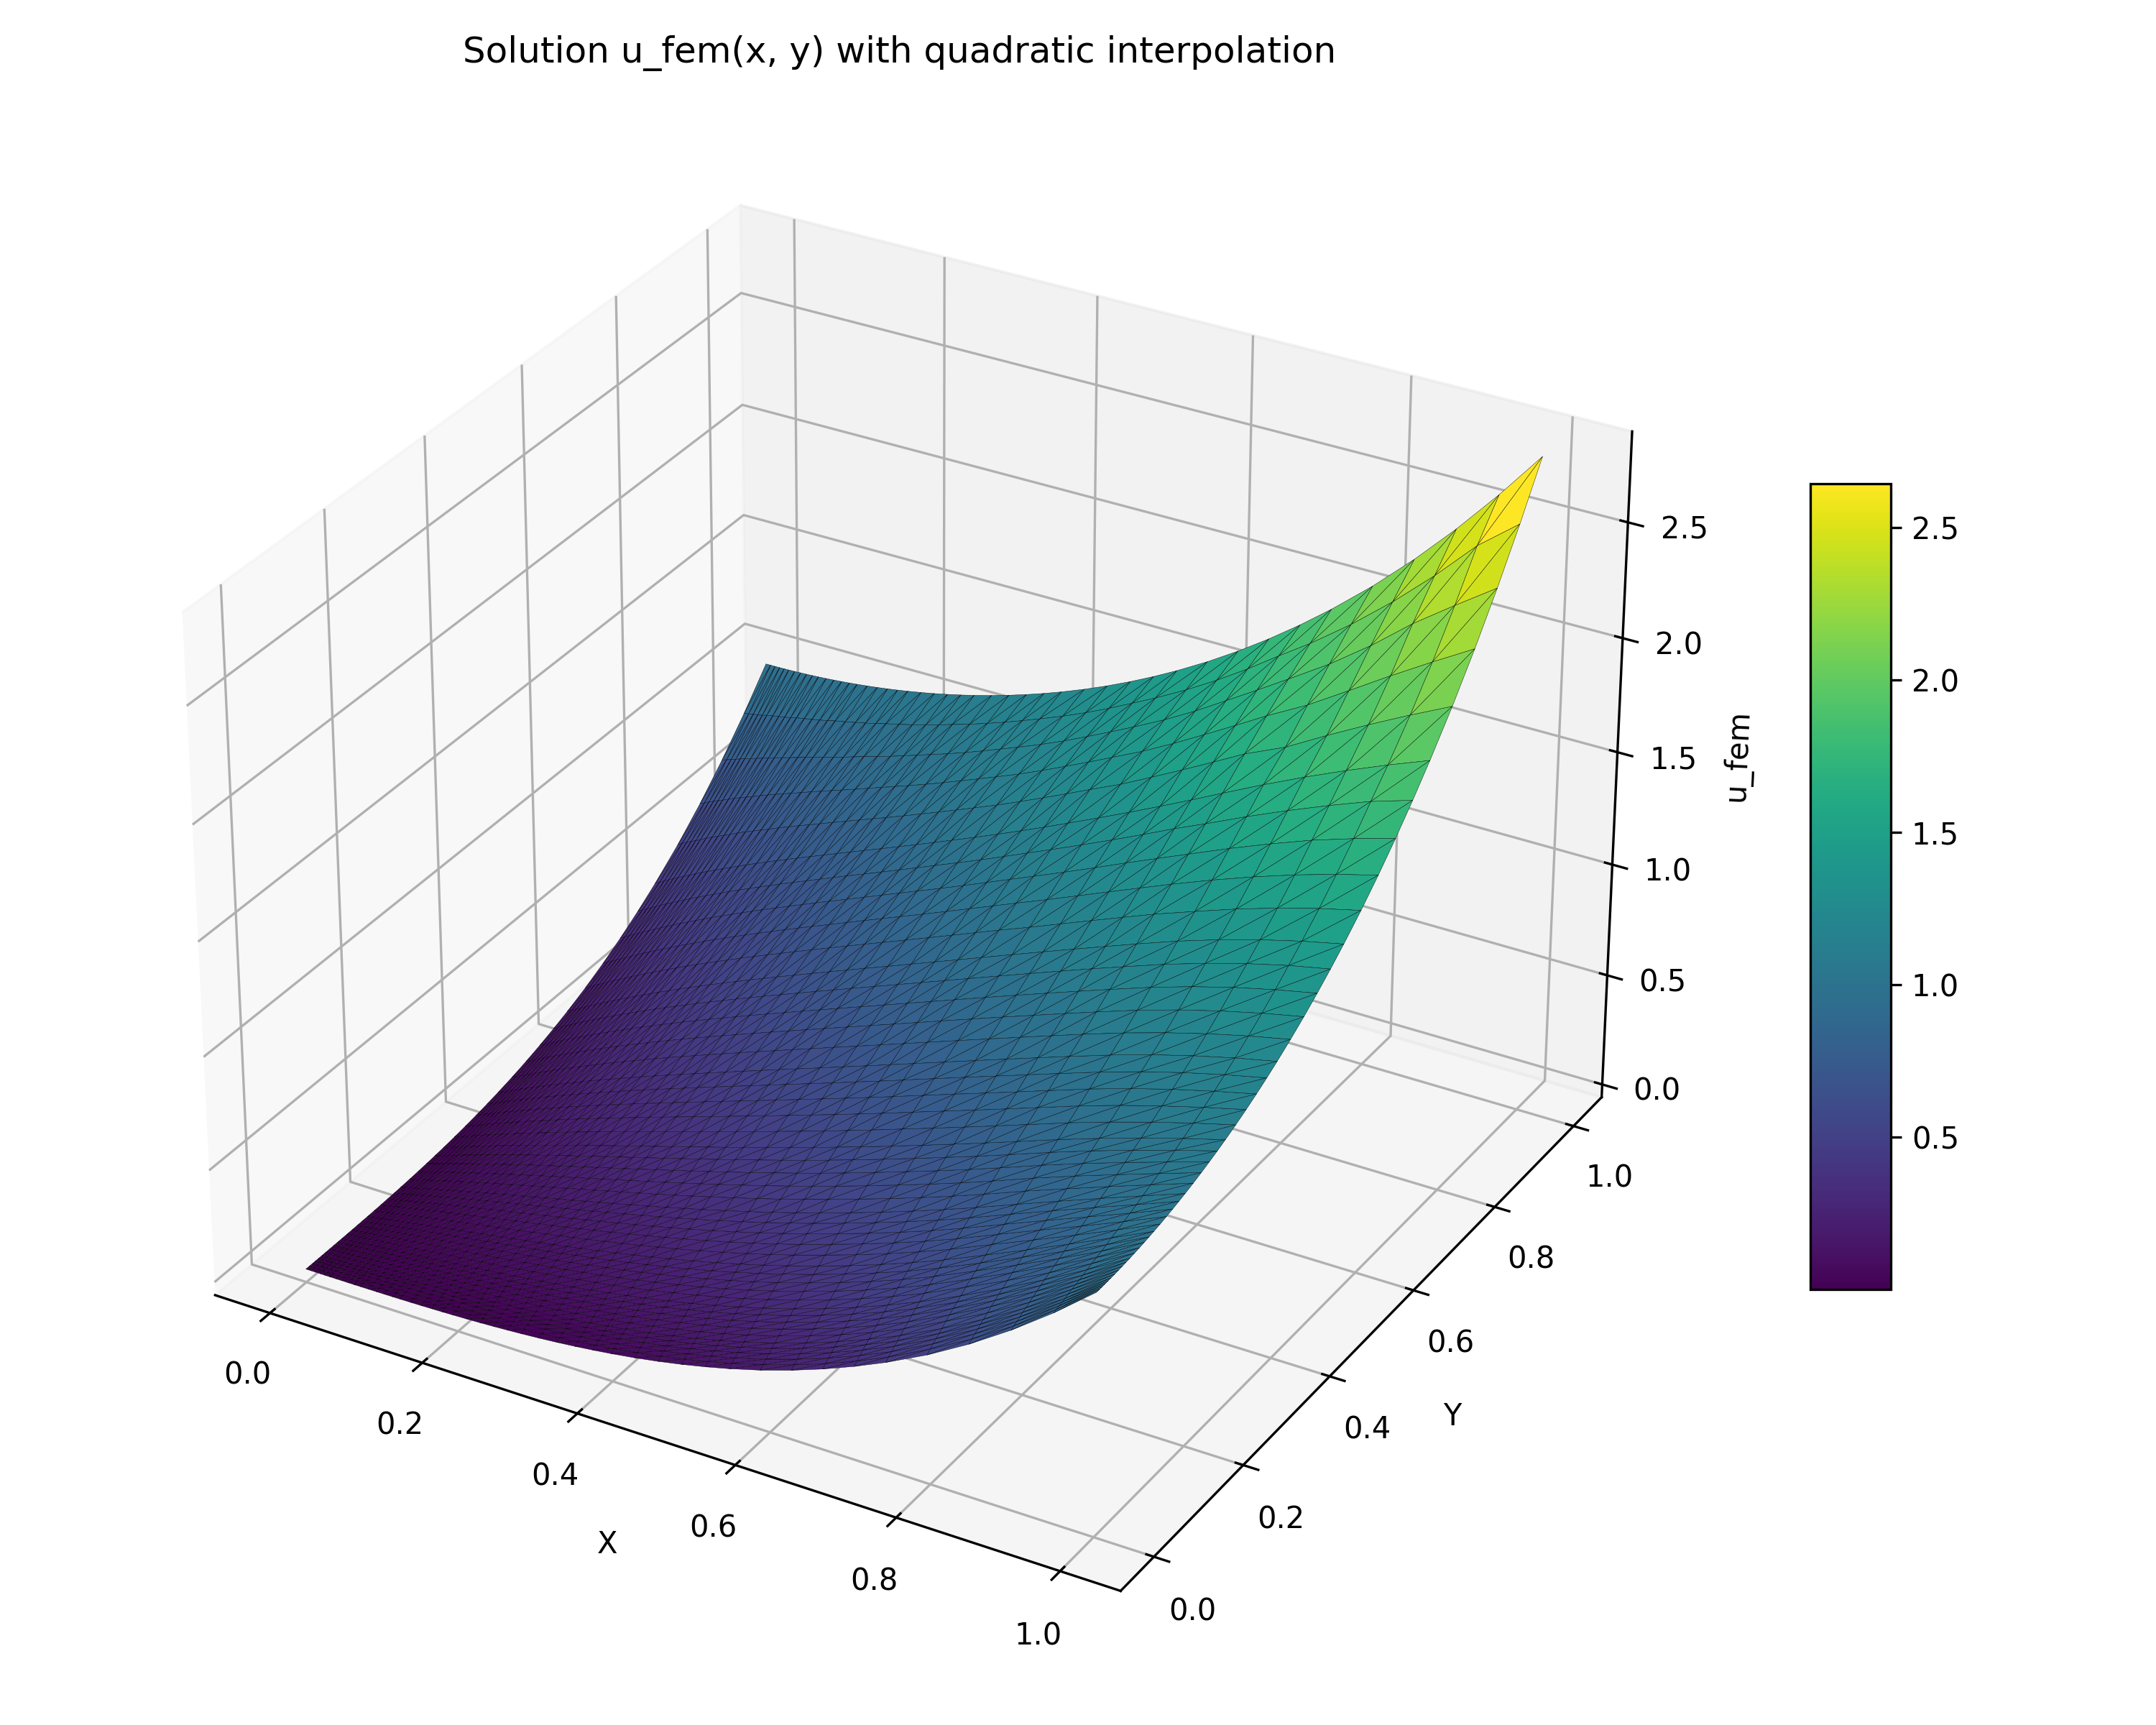
\includegraphics[width=\textwidth]{GRAFICOS/LST/LST_u_fem_sol_surface_plot.png}
    \caption{Discrete solution \(u_h\) for LST}
    \label{fig:lst_u_fem_sol}
  \end{subfigure}
  \hfill
  \begin{subfigure}[b]{0.48\textwidth}
    \centering
    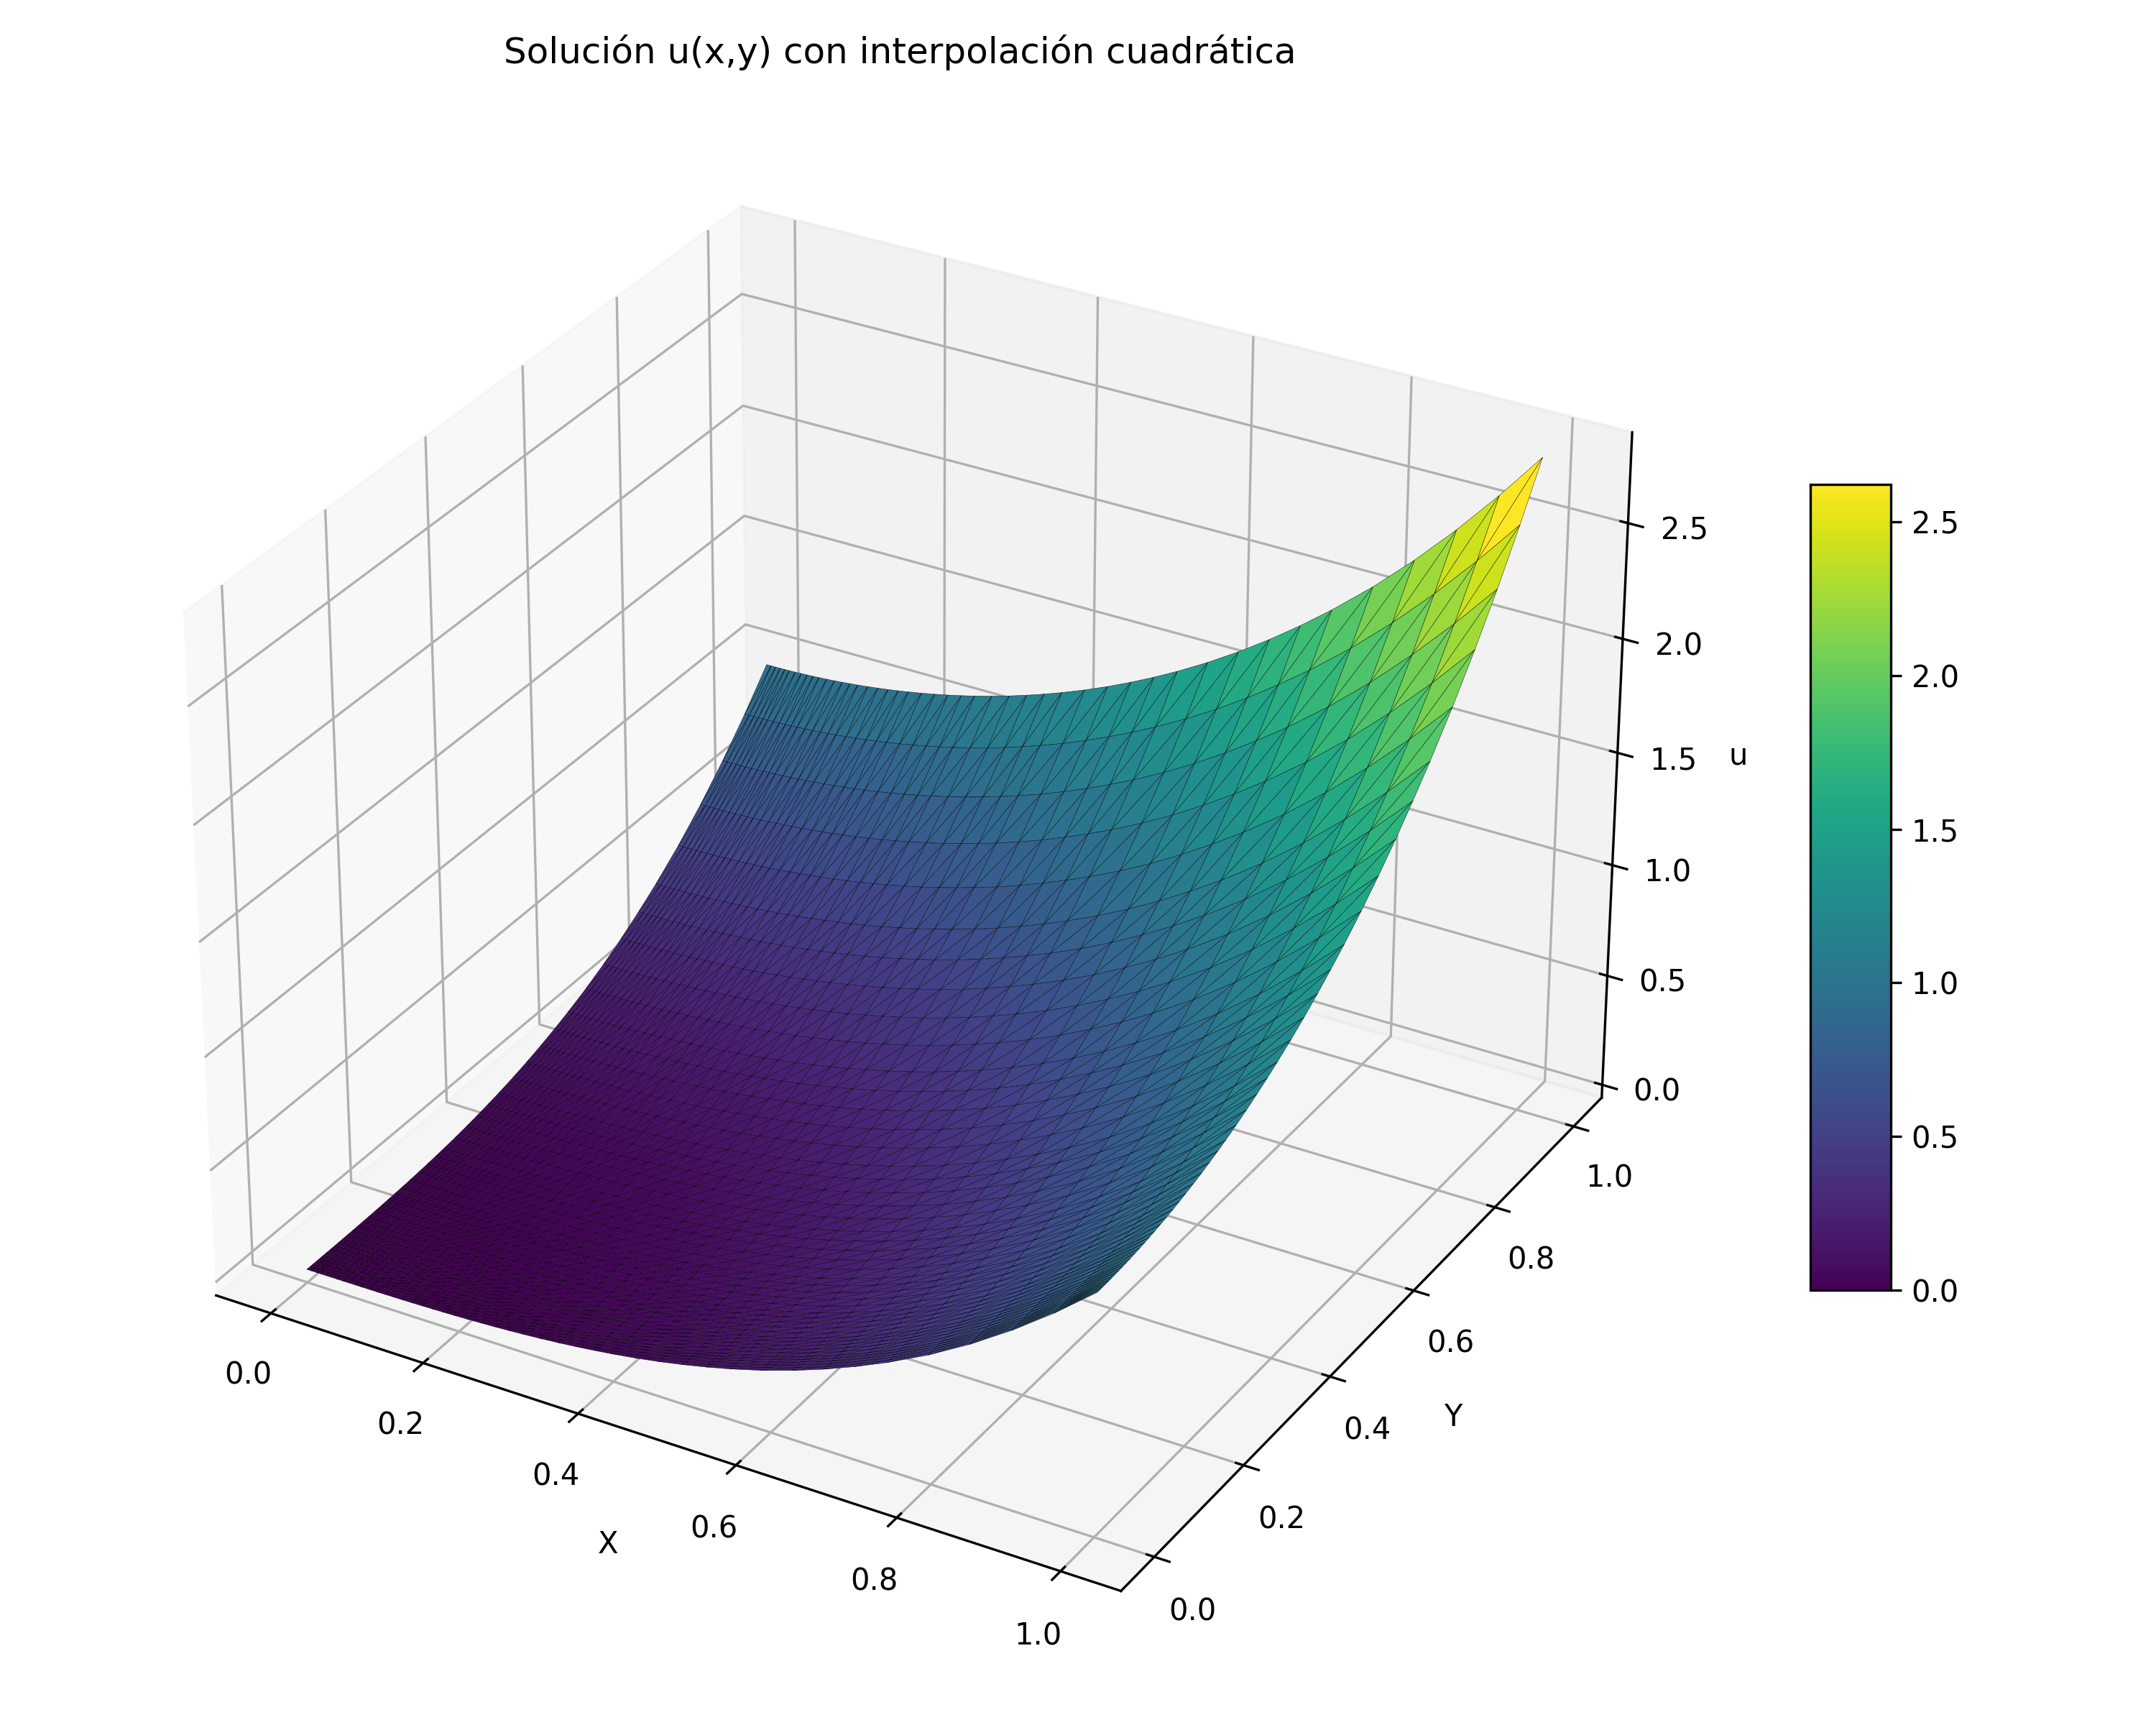
\includegraphics[width=\textwidth]{GRAFICOS/LST/LST_u_sol_surface_plot.png}
    \caption{Analytic solution \(u\) for LST}
    \label{fig:lst_error_plot}
  \end{subfigure}
  \caption{Comparison of the finite‐element discrete solution \(u_h\) and the analytic solution \(u\) for LST elements.}
  \label{fig:lst_comparison}
\end{figure}

\begin{figure}[H]
\centering
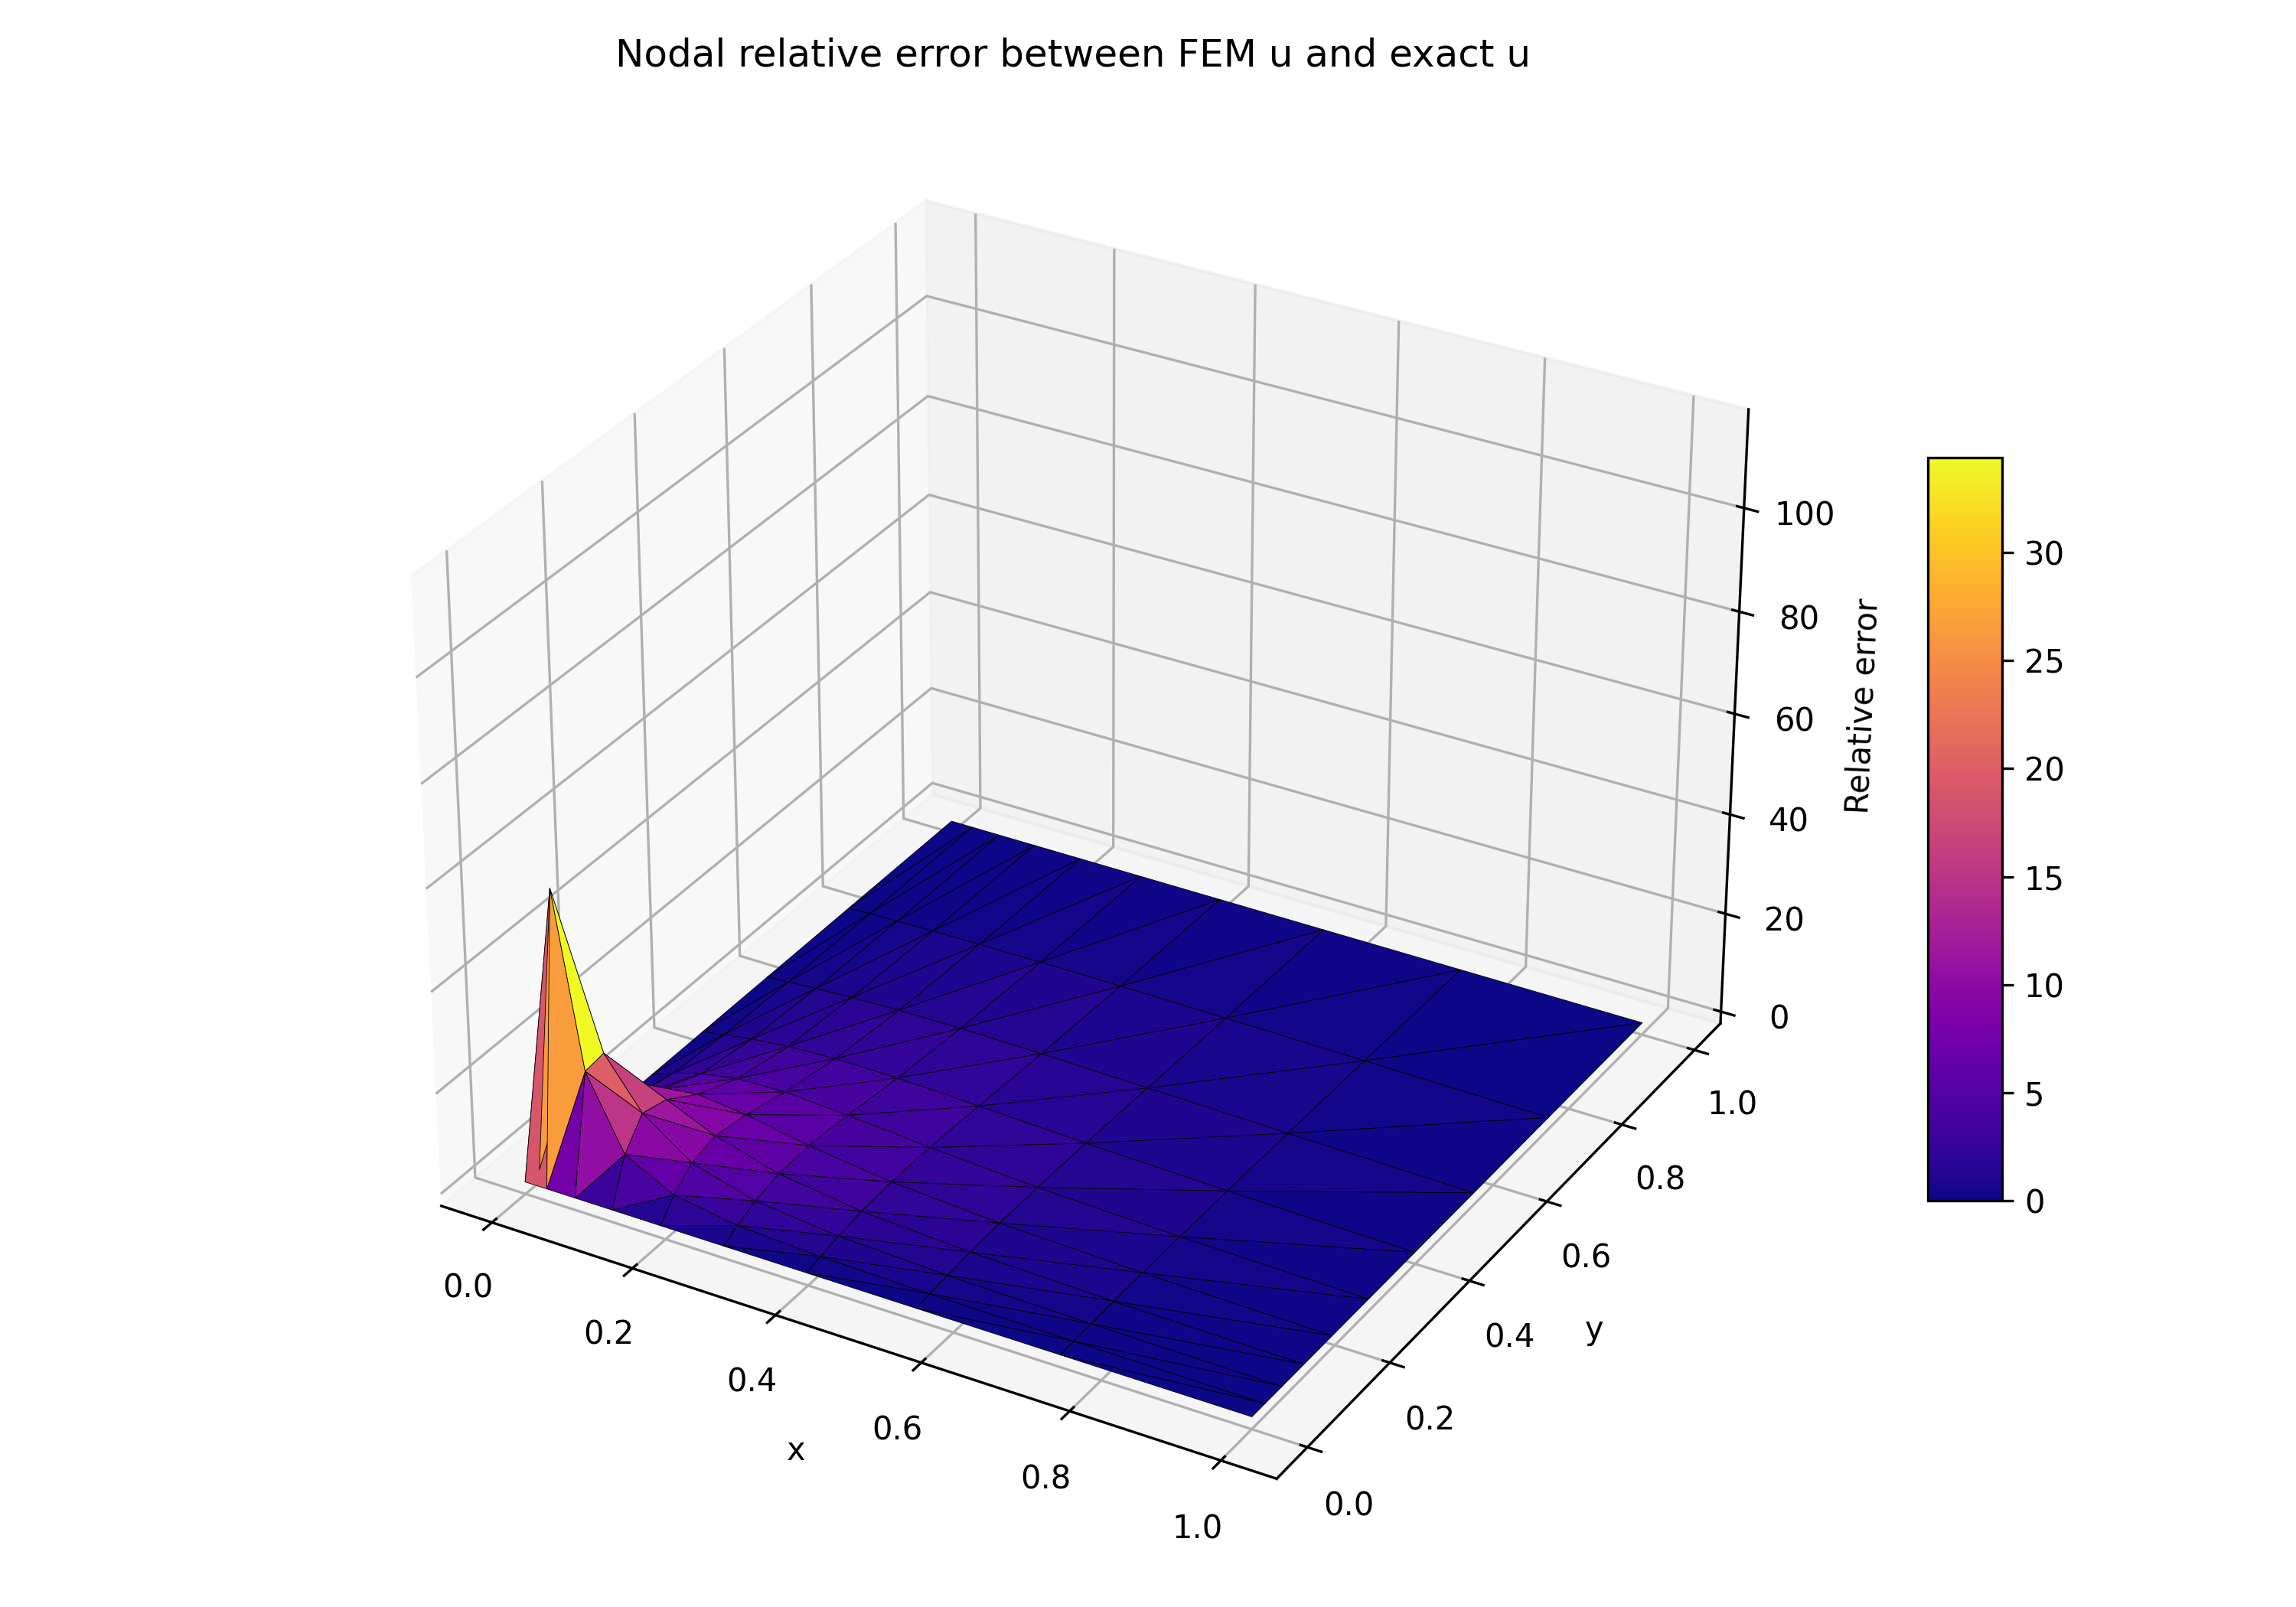
\includegraphics[width=0.6\textwidth]{GRAFICOS/LST/LST_relative_error_surface_plot.png}
\caption{Relative error \(\|u - u_h\|_{H^1(\Omega)}\) for LST elements}
\label{fig:lst_error_vs_h}
\end{figure}